\documentclass[11pt]{beamer}
\usetheme{Madrid}
\usepackage[utf8]{inputenc}
\usepackage[spanish]{babel}
\usepackage{amsmath}
\usepackage{amsfonts}
\usepackage{amssymb}
\usepackage{graphicx}
\usepackage{amsthm}
\newtheorem{defi}{Definición}
\newtheorem{eje}{Ejercicio}
\newtheorem{ejem}{Ejemplo}
\newtheorem{axiom}{Axioma}
\newtheorem{teor}{Teorema}
\usepackage{lipsum}
\author{Adriana Dávila Santos}
\title{Números Complejos}
%\setbeamercovered{transparent} 
%\setbeamertemplate{navigation symbols}{} 
%\logo{} 
%\institute{} 
%\date{} 
%\subject{} 
\begin{document}

\begin{frame}
\titlepage
\end{frame}

%\begin{frame}
%\tableofcontents
%\end{frame}

\begin{frame}{• Objetivo particular}
El alumno reconocerá de los números complejos las diferentes formas, realizará operaciones
fundamentales con ellos e identificará las propiedades de estas operaciones.
\end{frame}

\begin{frame}
\frametitle{Necesidad de los números complejos para la solución de ecuaciones de segundo grado: la
 unidad imaginaria}
\begin{defi}
\begin{center}
$\sqrt{-1}~=~i~\rightarrow~i^2~=~-1$, $i$ recibe el nombre de \textbf{unidad imaginaria}
\end{center}
\end{defi} 
Recordemos que hay ecuaciones de segundo grado, cuyas raíces no se encuentran en $\mathbb{R}$, ya que encontramos que la solución es la raíz cuadrada de un número negativo, por lo que nos salimos de los números reales para entrar al campo de los \textbf{complejos}.\\
Estos números surgen bajo la necesidad de poder dar respuesta a las raíces de números negativos, ya que muchas ecuaciones de n-ésimo grado las poseen.\\
Veamos esto con un ejemplo sencillo.
\end{frame}

\begin{frame}
\frametitle{Necesidad de los números complejos para la solución de ecuaciones de segundo grado: la
 unidad imaginaria}
\begin{ejem}
Encuentra las raíces de la ecuación $x^2=-4$\\
Resolveremos esta ecuación usando la fórmula general de 2º grado:\\ \hspace{0cm} \\
$x= \frac{-b~\pm ~\sqrt{b^2-4ac}}{2a} = \frac{-0~\pm ~\sqrt{0^2-4(1)(4)}}{2(1)} = \frac{0~\pm ~\sqrt{-16}}{2}$\\ \hspace{0cm} \\
Justo en este punto es dónde aparece la unidad imaginaria para resolver estos problemas, ya que tenemos lo siguiente:\\ \hspace{0cm} \\
$\frac{0~\pm ~\sqrt{(16) (-1)}}{2} = \frac{0~\pm ~\sqrt{16}\cdot \sqrt{-1}}{2} = \frac{0~\pm ~4i}{2} = \pm ~2i$\\ \hspace{0cm} \\
Como podemos observar, gracias a la unidad imaginaria, podemos obtener las raíces de este tipo de ecuaciones, en estos casos dónde aparece el número $i$, estamos hablando de números complejos.
\end{ejem}
\end{frame}

\begin{frame}
\frametitle{Forma binómica}
\framesubtitle{Estructura}
\begin{defi}
Definiremos al campo de los números complejos de la siguiente forma:\\ \hspace{0cm} \\
Sea $\mathbb{C} = \{z = a + bi : a,b\in \mathbb{R}~\&~i = \sqrt{-1}~(unidad~imaginaria)\}$\\ \hspace{0cm} \\
Dónde $'a'$ es la parte real y $'b'$ la imaginaria, si $b=0$, entonces estamos hablando de un número real
\end{defi}
\end{frame}

\begin{frame}
\frametitle{Forma binómica}
\framesubtitle{Suma y producto}
\begin{defi}
Definiremos al campo de los números complejos de la siguiente forma:\\ \hspace{0cm} \\
Sea $\mathbb{C} = \{z = a + bi : a,b\in \mathbb{R}~\&~i = \sqrt{-1}~(unidad~imaginaria)\}$\\ \hspace{0cm} \\
Dónde $a$ es la parte real y $b$ la imaginaria, si $b=0$, entonces estamos hablando de un número real
\end{defi}
\end{frame}

\begin{frame}
\frametitle{Forma binómica}
\framesubtitle{Suma y producto}
\begin{defi}
La suma (+) de números complejos en forma binómica consiste en operar las partes reales e imaginarias de manera independiente de la siguiente forma: \\
Sea $z_1 = a + bi$ y $z_2 = c + di$, $z + w = (a + c)+(b + d)i$
\end{defi}
\begin{defi}
El producto ($\cdot$) de números complejos en forma binómica, se trabaja de la misma forma que el producto de expresiones algebraicas, multiplicando cada número de un término con cada número del otro término y sumando respectivamente de la siguiente forma:\\ 
Sea $z_1 = a + bi$ y $z_2 = c + di$, $z_1 \cdot z_2 = (a+bi)(c+di) = (a\cdot c + a\cdot di + c\cdot bi + bi\cdot di)$\\
$\rightarrow z_1\cdot z_2 = (a\cdot c - b\cdot d) + (a\cdot d + c\cdot b)i$
\end{defi}
\end{frame}

\begin{frame}
\frametitle{Forma binómica}
\framesubtitle{Suma y producto}
\begin{ejem}
Sea $z_1 = 3 - 4i$ y $z_2 = 6 + 9i$\\ 
$z_1 + z_2 = (3 + 6)+(-4 + 9)i = 9 + 5i$
\end{ejem}
\begin{ejem}
Sea $z_3 = 5 + 2i$ y $z_4 = 12 + 7i$\\ 
$z_3 \cdot z_4 = (5+2i)(12+7i) = 5\cdot 12 + 5\cdot 7i + 12\cdot 2i + 2i\cdot 7i$\\
$z_3\cdot z_4 = 60+35i+24i-14 = 46+59i$\\
\end{ejem}
NOTA: Sea $x\in \mathbb{R}~y~z = (a+bi)\in \mathbb{C}$\\
$x(a+bi) = ax + bxi$
\end{frame}

\begin{frame}
\frametitle{Forma binómica}
\framesubtitle{Propiedades de la suma y el producto}
La suma posee la propiedad conmutativa, asociativa y de cerradura, existe el neutro aditivo ($0 + 0i = 0$) y existe el inverso aditivo $\forall z\in \mathbb{C} $ que es $-z$\\ \hspace{0cm} \\
El producto posee la propiedad conmutativa, asociativa y de cerradura, existe el neutro multiplicativo ($1 + 0i$) y existe el inverso multiplicativo $\forall z\in \mathbb{C} \neq 0$\\ \hspace{0cm} \\
El producto es distributivo sobre la suma de modo que:\\
$z_1(z_2+z_3)=z_1\cdot z_2 + z_1\cdot z_3~\forall z_i\in~\mathbb{C}$
\end{frame}

\begin{frame}
\frametitle{Forma binómica}
\framesubtitle{Conjugado y modulo de un número complejo}
\begin{defi}
El conjugado de un número complejo $z=a+bi$, denotado por $\bar{z}$, se define como $\bar{z}=a-bi$
\end{defi}
\begin{defi}
El modulo o valor absoluto de un número complejo $z=a+bi$, denotado por $|z|$, se define como $|z|=\sqrt{a^2+b^2}$
\end{defi}
\end{frame}

\begin{frame}
\frametitle{Forma binómica}
\framesubtitle{Conjugado y modulo de un número complejo}
\begin{teor}
Si un número $z\in \mathbb{C}$ es raíz de un polinomio o de una ecuación de n-ésimo grado $\rightarrow~\bar{z}$ también es raíz
\end{teor}
\begin{teor}
$\forall~z\in \mathbb{C},~z=a+bi$ se tiene que:\\
$z\cdot \bar{z} = z\cdot z = a^2+b^2$
\end{teor}
\begin{teor}
$\forall~z_1,~z_2\in \mathbb{C}$ se cumple que:\\
$\overline{(z_1+z_2)} = \overline{z_1}+\overline{z_2}$\\
$\overline{(z_1 \cdot z_2)} = \overline{z_1}\cdot \overline{z_2}$
\end{teor}
\end{frame}

\begin{frame}
\frametitle{Forma binómica}
\framesubtitle{Conjugado y modulo de un número complejo}
\begin{teor}
$\forall~z\in \mathbb{C}$, se tiene que: \\
$|z| \geq 0$, $|z| = 0 \Longleftrightarrow z = 0$
\end{teor}
\begin{teor}
$\forall~z_1,~z_2\in \mathbb{C}$, se cumple que: \\
$|z_1 \cdot z_2| = |z_1|\cdot |z_2|$
\end{teor}
\begin{eje}
Demostrar los teoremas anteriores
\end{eje}
\end{frame}

\begin{frame}
\frametitle{Forma binómica}
\framesubtitle{Conjugado y modulo de un número complejo}
\begin{ejem}
Determine el conjugado de los siguientes números complejos:\\
\begin{itemize}
\item $z_1 = -(2+5i)~\rightarrow~\overline{z_1} = -2+5i$
\item $z_2 = 18-3i~\rightarrow~\overline{z_1} = 18+3i$
\item $z_3 = -(-7+12i)~\rightarrow~\overline{z_1} = 7+12i$
\end{itemize}
\end{ejem}
\begin{ejem}
Determine el módulo de los siguientes números complejos:\\
\begin{itemize}
\item $z_1 = -(2+5i)~\rightarrow~|z_1| = \sqrt{(-2)^2+(-5)^2} = \sqrt{29}$
\item $z_2 = 18-3i~\rightarrow~|z_2| = \sqrt{(18)^2+(-3)^2} = \sqrt{333}$
\item $z_3 = -(-7+12i)~\rightarrow~|z_3| = \sqrt{(7)^2+(-12)^2} = \sqrt{193}$
\end{itemize}
\end{ejem}
\end{frame}

\begin{frame}
\frametitle{Forma binómica}
\framesubtitle{División}
\begin{defi}
Para dividir números complejos en forma binómica se multiplica numerador y denominador por el conjugado del denominador y se realizan las operaciones correspondientes. Sea $z_1 = a+bi,~z_2 = c+di~\rightarrow~z_1 \div z_2$ se resuelve de la siguiente forma: \\ \hspace{0cm} \\
$\frac{a+bi}{c+di} = \frac{(a+bi)(c-di)}{(c+di)(c-di)} = \frac{(ac+bd)+(bc-ad)i}{c^2+d^2} = \frac{ac+bd}{c^2+d^2}+\frac{bc-ad}{c^2+d^2}i$
\end{defi}
\begin{ejem}
$\frac{3+2i}{2+3i} = \frac{(3+2i)(2-3i)}{(2+3i)(2-3i)} = \frac{6-9i+4i+6}{4+9} = \frac{12}{13}-\frac{5}{13}i$
\end{ejem}
\end{frame}

\begin{frame}
\frametitle{Forma polar y exponencial}
\textbf{Forma polar: }
La forma polar de un número complejo es otra forma de representar un número complejo y se expresa como $z = r(cos(\theta) + isen(\theta))$, donde $r^2 = a^2+b^2~\rightarrow~r=|z|$\\
Esta forma se deduce del teorema de Pítagoras cómo se muestra a continuación, dónde '$x$' es el eje de los reales y '$y$' el de los imaginarios:\\ \hspace{0cm} \\
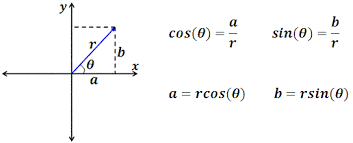
\includegraphics[scale=0.75]{polar.jpg}\\
Por último vemos que $\theta = tan^{-1}(\frac{b}{a})$ 
\end{frame}

\begin{frame}
\frametitle{Forma polar y exponencial}
\textbf{Forma exponencial: }
Para representar a un número complejo a su forma exponencial debemos expresarlo de la siguiente forma: \\
\begin{center}
$z = re^{i\theta}$\\
\end{center}
De dónde ya sabemos que $e = 2.7182818...$, $r = |z|$ y que $\theta = tan^{-1}(\frac{b}{a})$
\end{frame}

\begin{frame}
\frametitle{Forma polar y exponencial}
\framesubtitle{ Conversión de números complejos en sus diferentes formas}
\begin{ejem}
Pasar el número $z = 2+2i$ a su forma polar y exponencial\\
\textbf{Forma polar:}\\ \hspace{0cm} \\
$r = |z| = \sqrt{a^2 + b^2} = \sqrt{2^2 + 2^2} = \sqrt{4 + 4} = \sqrt{8} = 2\sqrt{2}$\\ \hspace{0cm} \\
$\theta = tan{-1}(\frac{b}{a}) = tan{-1}(\frac{2}{2}) = tan{-1}(1) =  45^o = \frac{\pi}{4}rad$\\ \hspace{0cm} \\
$\rightarrow~z = 2\sqrt{2}[cos(\frac{\pi}{4}) + isen(\frac{\pi}{4})]$\\ \hspace{0cm} \\
\textbf{Forma exponencial:}\\ \hspace{0cm} \\
$z = re^{i\theta} = 2\sqrt{2}(e^{\frac{\pi}{4}i})$\\
\end{ejem}
NOTA: Se recomienda trabajar los ángulos en radianes
\end{frame}

\begin{frame}
\frametitle{Forma polar y exponencial}
\framesubtitle{Conjugado en forma polar y en forma exponencial}
\begin{eje}
Sea el número complejo $z = r[cos(\theta)+isen(\theta)]$. Demostrar que $\overline{z} = r[cos(\theta)-isen(\theta)]$
\end{eje}
\begin{eje}
Sea el número complejo $z = r(e^{i\theta})$. Demostrar que $\overline{z} = r(e^{-i\theta})$
\end{eje}
\end{frame}

\begin{frame}
\frametitle{Forma polar y exponencial}
\framesubtitle{Conjugado en forma polar y en forma exponencial}
\begin{ejem}
Sea el número complejo $z = 2\sqrt{2}[cos(\frac{\pi}{4})+isen(\frac{\pi}{4})]$, determine su conjugado.\\
$\overline{z} = 2\sqrt{2}[cos(\frac{\pi}{4})-isen(\frac{\pi}{4})]$
\end{ejem}
\begin{ejem}
Sea el número complejo $z = 2\sqrt{2}(e^{\frac{\pi}{4}i})$, determine su conjugado.\\
$z = 2\sqrt{2}(e^{-\frac{\pi}{4}i})$
\end{ejem}
\end{frame}

\begin{frame}
\frametitle{Forma polar y exponencial}
\framesubtitle{Producto y división en forma polar y en forma exponencial}
\textbf{Multiplicación forma polar:}\\ \hspace{0cm} \\
Sea $z_1 = r_1[cos(\theta_1) + isen(\theta_1)]$ y $z_2 = r_2[cos(\theta_2) + isen(\theta_2)]$\\ \hspace{0cm} \\
$\rightarrow~z_1\cdot z_2 = r_1\cdot r_2[cos(\theta_1 + \theta_2) + isen(\theta_1 + \theta_2)]$\\ \hspace{0cm} \\
\textbf{Multiplicación forma exponencial:}\\ \hspace{0cm} \\
Sea $z_1 = r_1(e^{i\theta_1})$ y $z_2 = r_2(e^{i\theta_2})$\\ \hspace{0cm} \\
$\rightarrow~z_1\cdot z_2 = r_1\cdot r_2[e^{i(\theta_1+\theta_2)}]$
\end{frame}

\begin{frame}
\frametitle{Forma polar y exponencial}
\framesubtitle{Producto y división en forma polar y en forma exponencial}
\begin{ejem}
Sea $z_1 = 3\sqrt{2}[cos(\frac{\pi}{4}) + isen(\frac{\pi}{4})]$ y $z_2 = 2\sqrt{2}[cos(\frac{\pi}{2}) + isen(\frac{\pi}{2})]$\\ \hspace{0cm} \\
$\rightarrow~z_1\cdot z_2 = (3\sqrt{2})(2\sqrt{2})[cos(\frac{\pi}{4}+\frac{\pi}{2}) + isen(\frac{\pi}{4}+\frac{\pi}{2})] = 
12[cos(\frac{3\pi}{4}) + isen(\frac{3\pi}{4})]$
\end{ejem}
\begin{ejem}
Sea $z_1 = 3\sqrt{2}(e^{i\frac{\pi}{4}})$ y $z_2 = 2\sqrt{2}(e^{i\frac{\pi}{2}})$\\ \hspace{0cm} \\
$\rightarrow~z_1\cdot z_2 = (3\sqrt{2})(2\sqrt{2})[e^{i(\frac{\pi}{4}+\frac{\pi}{2})}] = 12(e^{i\frac{3\pi}{4}})$
\end{ejem}
\end{frame}

\begin{frame}
\frametitle{Forma polar y exponencial}
\framesubtitle{Producto y división en forma polar y en forma exponencial}
\textbf{División forma polar:}\\ \hspace{0cm} \\
Sea $z_1 = r_1[cos(\theta_1) + isen(\theta_1)]$ y $z_2 = r_2[cos(\theta_2) + isen(\theta_2)]$\\ \hspace{0cm} \\
$\rightarrow~z_1\div z_2 = \frac{r_1}{r_2}[cos(\theta_1 - \theta_2) + isen(\theta_1 - \theta_2)]$\\ \hspace{0cm} \\
\textbf{División forma exponencial:}\\ \hspace{0cm} \\
Sea $z_1 = r_1(e^{i\theta_1})$ y $z_2 = r_2(e^{i\theta_2})$\\ \hspace{0cm} \\
$\rightarrow~z_1\div z_2 = \frac{r_1}{r_2}(e^{i(\theta_1 - \theta_2)})$
\end{frame}

\begin{frame}
\frametitle{Forma polar y exponencial}
\framesubtitle{Producto y división en forma polar y en forma exponencial}
\begin{ejem}
Sea $z_1 = 3\sqrt{2}[cos(\frac{\pi}{2}) + isen(\frac{\pi}{2})]$ y $z_2 = 2\sqrt{2}[cos(\frac{\pi}{4}) + isen(\frac{\pi}{4})]$\\ \hspace{0cm} \\
$\rightarrow~z_1\div z_2 = \frac{3\sqrt{2}}{2\sqrt{2}}[cos(\frac{\pi}{2}-\frac{\pi}{4}) + isen(\frac{\pi}{2}-\frac{\pi}{4})] = 
\frac{3}{2}[cos(\frac{\pi}{4}) + isen(\frac{\pi}{4})]$
\end{ejem}
\begin{ejem}
Sea $z_1 = 3\sqrt{2}(e^{i\frac{\pi}{2}})$ y $z_2 = 2\sqrt{2}(e^{i\frac{\pi}{4}})$\\ \hspace{0cm} \\
$\rightarrow~z_1\div z_2 = \frac{3\sqrt{2}}{2\sqrt{2}}(e^{i(\frac{\pi}{4}-\frac{\pi}{2})}) = \frac{3}{2}(e^{i\frac{\pi}{4}})$
\end{ejem}
\end{frame}

\begin{frame}
\frametitle{Forma polar y exponencial}
\framesubtitle{Solución de ecuaciones}
Para resolver una ecuación de n-ésimo grado debemos tener en cuenta que existen n soluciones, en el caso de los números complejos debemos trabajarlos en forma polar o exponencial para poder hallar las raíces. \\
Recordemos que en un número complejo $z = r[cos(\theta)+isen(\theta)]$, \textbf{r} es el módulo y \textbf{$\theta$} es el ángulo o argumento. \\
Al obtener las raíces del número complejo z, por lo general el módulo se va a mantener constante, sin embargo, el ángulo o argumento es el que va a cambiar y el que hará que las soluciones sean distintas.\\
Para obtener los ángulos lo haremos de manera iterativa con la siguiente fórmula:\\
\begin{center}
$\theta_k = \frac{\theta + 2\pi k}{n}$\\
\end{center}
Donde k = \{0,1,2,...,n-1\} y n es la raíz o potencia de z
\end{frame}

\begin{frame}
\frametitle{Forma polar y exponencial}
\framesubtitle{Solución de ecuaciones}
\begin{ejem}
Resuelva la ecuación $z^4+1=0$\\
Primero despejamos z de la siguiente forma:\\
\begin{center}
$z^4=-1$\\
$z^4= 1[cos(\pi)+isen(\pi)]$\\
$z = (cos(\pi)+isen(\pi))^\frac{1}{4}$\\
\end{center}
Al ser una ecuación de cuarto grado, obtendremos cuatro raíces, así que comenzamos a obtenerlas de manera iterativa:\\
\begin{center}
$z_0 = \sqrt[4]{1}[cos(\frac{\pi + 2\pi \cdot 0}{4})+isen(\frac{\pi + 2\pi \cdot 0}{4})] = 
[cos(\frac{\pi}{4})+isen(\frac{\pi}{4})]$\\ \hspace{0cm} \\
$z_1 = \sqrt[4]{1}[cos(\frac{\pi + 2\pi \cdot 1}{4})+isen(\frac{\pi + 2\pi \cdot 1}{4})] = 
[cos(\frac{3\pi}{4})+isen(\frac{3\pi}{4})]$\\ \hspace{0cm} \\
\end{center}
\end{ejem}
\end{frame}

\begin{frame}
\frametitle{Forma polar y exponencial}
\framesubtitle{Solución de ecuaciones}
\begin{ejem}
$z_2 = \sqrt[4]{1}[cos(\frac{\pi + 2\pi \cdot 2}{4})+isen(\frac{\pi + 2\pi \cdot 2}{4})] = 
[cos(\frac{5\pi}{4})+isen(\frac{5\pi}{4})]$\\ \hspace{0cm} \\
$z_3 = \sqrt[4]{1}[cos(\frac{\pi + 2\pi \cdot 3}{4})+isen(\frac{\pi + 2\pi \cdot 3}{4})] = 
[cos(\frac{7\pi}{4})+isen(\frac{7\pi}{4})]$\\ \hspace{0cm} \\
\end{ejem}
De este modo obtenemos las 4 soluciones, si continuaramos iterando con $z_4$ observariamos que el resultado sería igual a $z_0$, por lo que se convertiría en un ciclo.\\
Las raíces están expresadas en forma polar, sin embargo pueden pasarse a forma exponencial o binómica:\\
\begin{itemize}
\item $z_0 = e^{i\frac{\pi}{4}}$
\item $z_1 = e^{i\frac{3\pi}{4}}$
\item $z_2 = e^{i\frac{5\pi}{4}}$
\item $z_3 = e^{i\frac{7\pi}{4}}$
\end{itemize}
\end{frame}

\begin{frame}
\frametitle{Forma polar y exponencial}
\framesubtitle{Solución de ecuaciones}
\begin{ejem}
Resuelva la ecuación $z^4=-8+8\sqrt{3}i$\\
Primero despejamos z de la siguiente forma:\\
\begin{center}
$z^4=16[cos(\frac{2\pi}{3})isen(\frac{2\pi}{3})]$\\
$z = 16[cos(\frac{2\pi}{3})isen(\frac{2\pi}{3})]^\frac{1}{4}$\\
\end{center}
Al ser una ecuación de cuarto grado, obtendremos cuatro raíces, así que comenzamos a obtenerlas de manera iterativa:\\
\begin{center}
$z_0 = \sqrt[4]{16}[cos(\frac{\frac{2\pi}{3}+2\pi \cdot 0}{4})+isen(\frac{\frac{2\pi}{3}+2\pi \cdot 0}{4})]^\frac{1}{4} = 
2[cos(\frac{\pi}{6})+isen(\frac{\pi}{6})]$\\ \hspace{0cm} \\
$z_1 = \sqrt[4]{16}[cos(\frac{\frac{2\pi}{3}+2\pi \cdot 1}{4})+isen(\frac{\frac{2\pi}{3}+2\pi \cdot 1}{4})]^\frac{1}{4} = 
2[cos(\frac{2\pi}{3})+isen(\frac{2\pi}{3})]$\\ \hspace{0cm} \\
\end{center}
\end{ejem}
\end{frame}

\begin{frame}
\frametitle{Forma polar y exponencial}
\framesubtitle{Solución de ecuaciones}
\begin{ejem}
$z_2 = \sqrt[4]{16}[cos(\frac{\frac{2\pi}{3}+2\pi \cdot 2}{4})+isen(\frac{\frac{2\pi}{3}+2\pi \cdot 2}{4})]^\frac{1}{4} = 
2[cos(\frac{7\pi}{6})+isen(\frac{7\pi}{6})]$\\ \hspace{0cm} \\
$z_3 = \sqrt[4]{16}[cos(\frac{\frac{2\pi}{3}+2\pi \cdot 3}{4})+isen(\frac{\frac{2\pi}{3}+2\pi \cdot 3}{4})]^\frac{1}{4} = 
2[cos(\frac{5\pi}{3})+isen(\frac{5\pi}{3})]$\\ \hspace{0cm} \\
\begin{itemize}
\item $z_0 = 2e^{i\frac{\pi}{6}}$
\item $z_1 = 2e^{i\frac{2\pi}{3}}$
\item $z_2 = 2e^{i\frac{7\pi}{6}}$
\item $z_3 = 2e^{i\frac{5\pi}{3}}$
\end{itemize}
\end{ejem}
\end{frame}

\end{document}